\section{Experiments and Results}
\label{sec:experiments}
\label{sec:model-evaluation}
\begingroup
\setlength{\emergencystretch}{3em}

\subsection{Experimental Setup}
\label{subsec:exp-setup}

The 2,397,001 cleaned listings are split by publication date into 70\% training (June--December 2025), 15\% validation (December 2025--January 2026), and 15\% test (January--March 2026). Models are tuned on the validation set, and all reported results are computed on the test set.

During training, models predict $\log(1 + \text{price})$; predictions are transformed back to VND before calculating errors. Performance is measured by MAE and RMSE (in billion VND), $R^2$, and MAPE (\%).

\subsection{Overall Performance}
\label{subsec:overall-results}

Table~\ref{tab:all-model-results} and Figure~\ref{fig:model-comparison} present the complete test-set comparison across 11 individual models and four blends.

\begin{table}[H]
\centering
\caption[Complete test-set comparison]{Test-set performance across all evaluated models and blends. MAE and RMSE are measured in billion VND; bold values indicate the best overall result.}
\label{tab:all-model-results}
\small
\renewcommand{\arraystretch}{1.1}
\begin{tabularx}{\textwidth}{Xrrrr}
\toprule
Model & MAE & RMSE & $R^2$ & MAPE (\%) \\
\midrule
Median-price baseline & 11.700 & 36.650 & -0.059 & 98.29 \\
Local median price per m$^2$ & 7.225 & 42.901 & -0.451 & 47.35 \\
Structured Ridge & 5.730 & 23.865 & 0.551 & 31.97 \\
\midrule
Random Forest & 5.406 & 22.063 & 0.616 & 31.22 \\
LightGBM & 4.464 & 18.189 & 0.739 & 26.24 \\
CatBoost & 5.242 & 21.065 & 0.650 & 31.66 \\
XGBoost & 4.485 & 18.401 & 0.733 & 26.42 \\
\midrule
Ridge with TF-IDF & 4.935 & 21.606 & 0.632 & 28.09 \\
LightGBM + text prediction & 4.223 & 17.317 & 0.764 & 25.05 \\
MLP + embeddings & 4.620 & 19.264 & 0.707 & 26.83 \\
BamiBERT (text only) & 4.355 & 17.353 & 0.763 & 26.86 \\
\midrule
Structured blend & 4.241 & 17.357 & 0.762 & 25.90 \\
Structured + TF-IDF blend & 4.025 & 17.020 & 0.772 & 24.31 \\
Structured + BamiBERT blend & 3.699 & 16.283 & 0.791 & 21.94 \\
\textbf{All-model blend} & \textbf{3.659} & \textbf{16.171} & \textbf{0.794} & \textbf{21.70} \\
\bottomrule
\end{tabularx}
\end{table}

\begin{figure}[H]
\centering
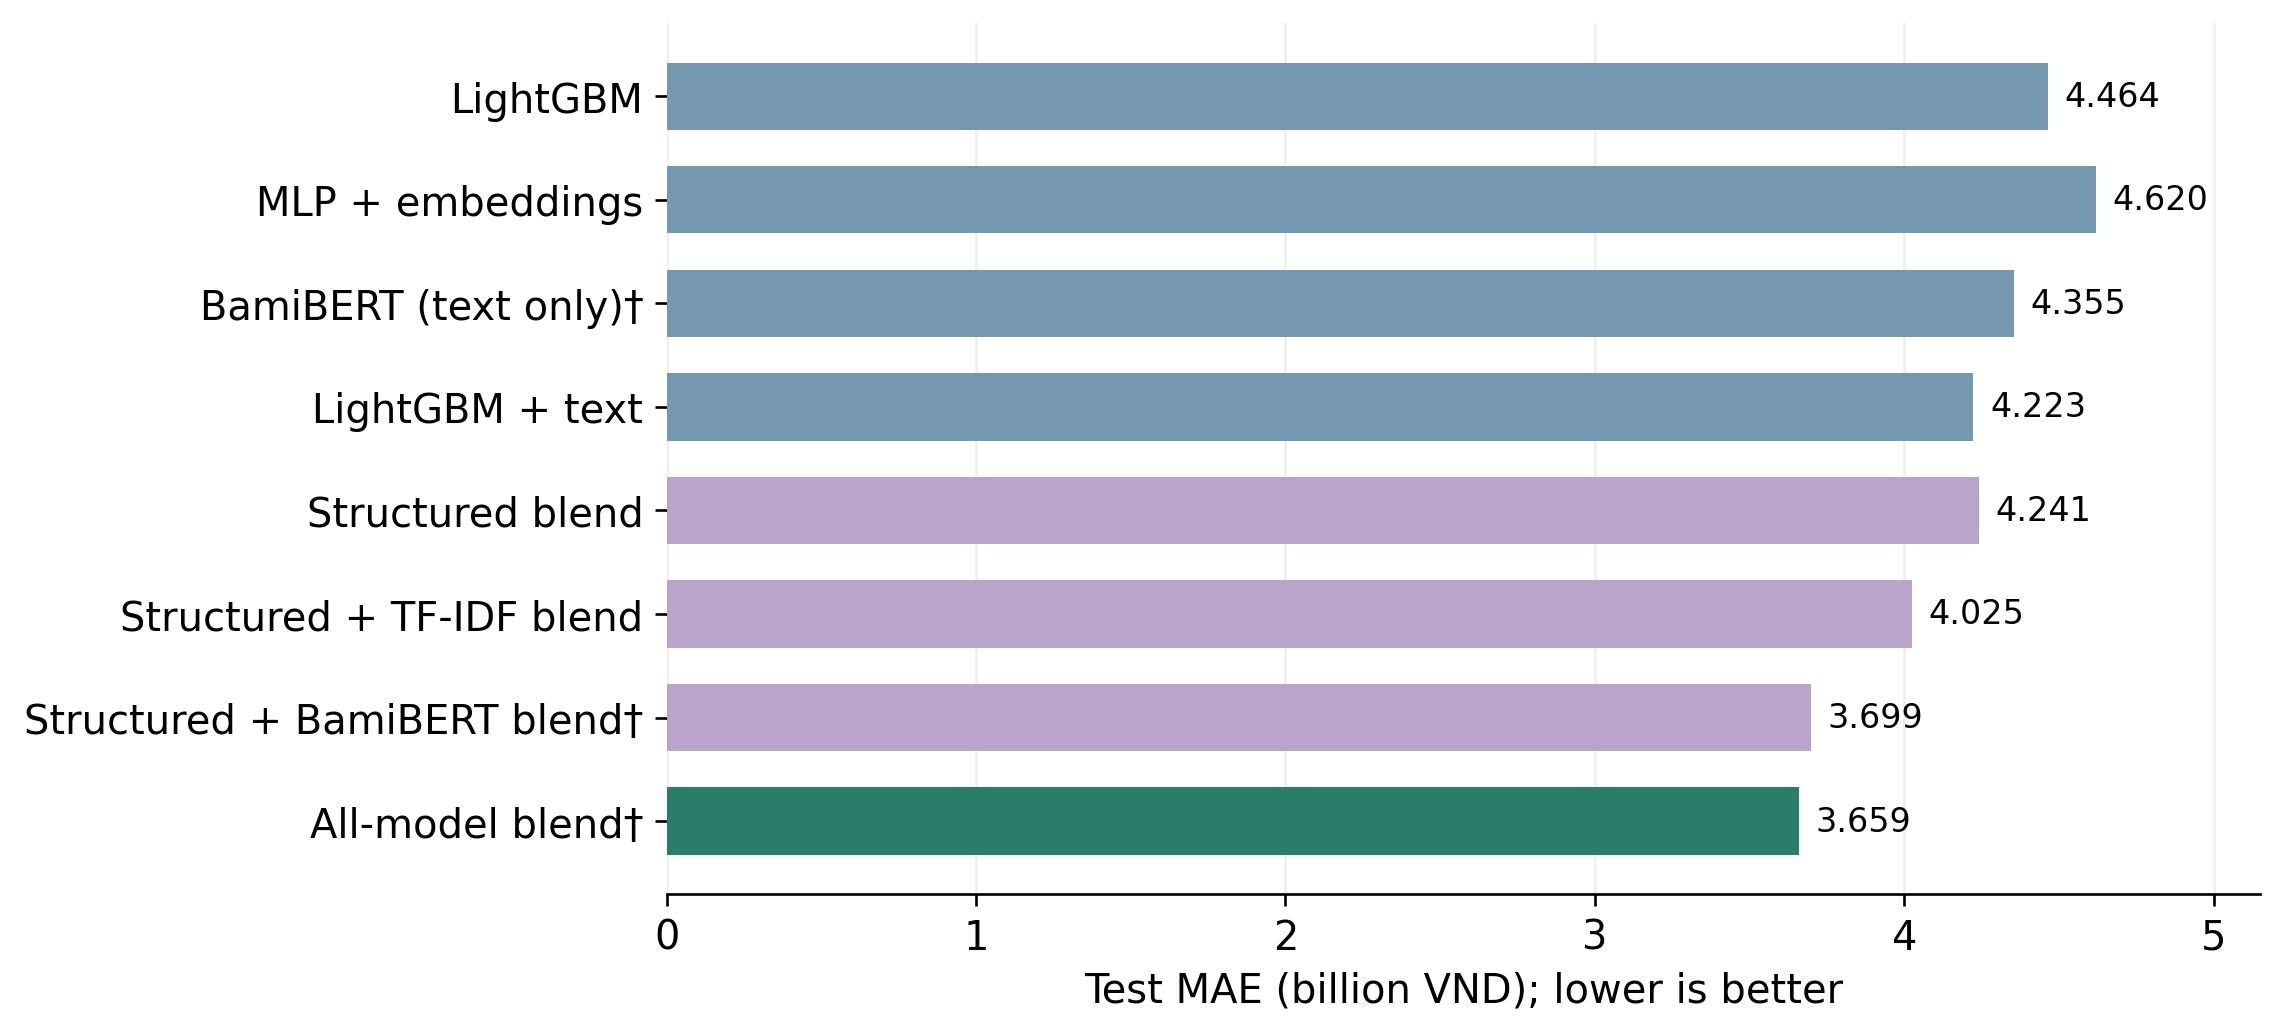
\includegraphics[width=0.82\textwidth]{figures/conclusion_model_comparison.png}
\caption[Test MAE of models and combinations]{Test MAE across selected predictors and blends (lower is better).}
\label{fig:model-comparison}
\end{figure}

The evaluated approaches fall into four distinct tiers of performance:
\begin{enumerate}
  \item \textbf{Naive baselines:} Direct median predictions produce large errors ($\text{MAE} > 7$ billion VND).
  \item \textbf{Linear and shallow ensembles:} Ridge regression, Random Forest, and CatBoost form an intermediate group with MAE between 5.2 and 5.7 billion VND.
  \item \textbf{High-capacity individual models:} Scaled gradient-boosted trees (LightGBM, XGBoost), the deep tabular MLP, and text models (TF-IDF enhanced LightGBM and BamiBERT) cluster tightly between 4.2 and 4.6 billion VND.
  \item \textbf{Multi-modal prediction blends:} Stacking models across structured and textual modalities yields the strongest results, reaching an MAE of 3.659 billion VND.
\end{enumerate}

In absolute terms, prediction errors remain sizable. An MAE of 3.659 billion VND is substantial given typical property prices between 1 and 10 billion VND. Furthermore, RMSE is more than four times larger than MAE across all models, reflecting extreme squared errors driven by luxury and high-value properties in the distribution tail.

\subsection{Performance Analysis by Model Family and Modality}
\label{subsec:detailed-analysis}

\subsubsection{Baselines and Linear Regression}

Predicting the training median asking price yields an MAE of 11.700 billion VND and $R^2=-0.059$. Scaling local district-level median prices per square metre reduces MAE to 7.225 billion VND, but inflates RMSE to 42.901 billion VND ($R^2=-0.451$). Because this heuristic scales linearly with area, it incurs severe errors on unusually large parcels or luxury properties.

Ridge regression~\cite{hoerl1970ridge} on structured attributes establishes the first viable predictive baseline (MAE 5.730 billion VND, $R^2=0.551$). As shown in Figure~\ref{fig:ml-ridge-diagnostic}, while predictions for mid-range properties align well with actual values, the model substantially underestimates high-end properties.

\begin{figure}[H]
\centering
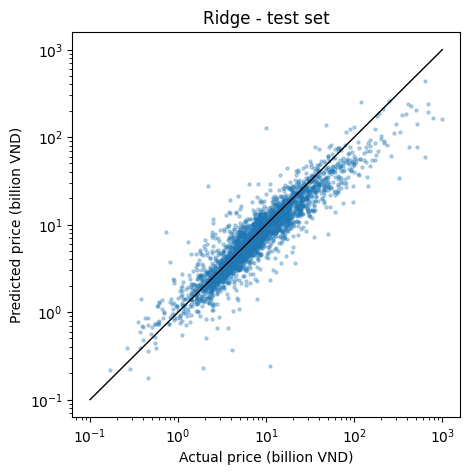
\includegraphics[width=0.60\textwidth]{figures/ml_ridge_actual_vs_predicted.png}
\caption[Ridge: actual vs.\ predicted prices]{Actual vs.\ predicted asking prices for 3,000 test listings under structured Ridge. Both axes are logarithmic in billion VND; the diagonal marks exact agreement.}
\label{fig:ml-ridge-diagnostic}
\end{figure}

\subsubsection{Tree Ensembles}

Nonlinear decision-tree ensembles yield significant improvements over Ridge. Random Forest~\cite{breiman2001forests} attains an MAE of 5.406 billion VND. Gradient-boosted trees perform best among purely structured models: LightGBM~\cite{ke2017lightgbm} (MAE 4.464, $R^2=0.739$) and XGBoost~\cite{chen2016xgboost} (MAE 4.485, $R^2=0.733$) perform almost identically, cutting MAE by approximately 22\% relative to Ridge. CatBoost~\cite{prokhorenkova2018catboost} performs closer to Random Forest (MAE 5.242, $R^2=0.650$).

\begin{figure}[htbp]
\centering
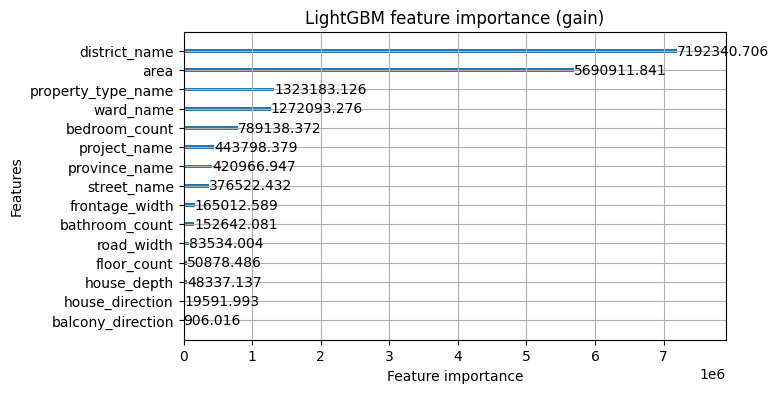
\includegraphics[width=0.90\textwidth]{figures/ml_lightgbm_feature_importance.png}
\caption[LightGBM feature importance]{LightGBM feature importance by accumulated split gain.}
\label{fig:ml-lightgbm-importance}
\end{figure}

Figure~\ref{fig:ml-lightgbm-importance} illustrates the split-gain importance ranking from LightGBM. The signal is heavily concentrated in geographical location (district, ward) and property size (area), followed by property category and bedroom count. Secondary physical attributes, including house and balcony direction, provide negligible predictive gain.

\subsubsection{Tabular Neural Network (MLP)}

The tabular MLP with categorical embeddings~\cite{gorishniy2021revisiting} achieves an MAE of 4.620 billion VND and $R^2=0.707$. It outperforms linear regression and Random Forest, but does not match the performance of LightGBM or XGBoost. This aligns with empirical benchmarks showing that gradient boosting remains challenging to outperform on heterogeneous tabular datasets~\cite{gorishniy2021revisiting}. As shown in Figure~\ref{fig:dl-mlp-training}, validation error converged smoothly and reached its minimum at epoch 10.

\begin{figure}[htbp]
\centering
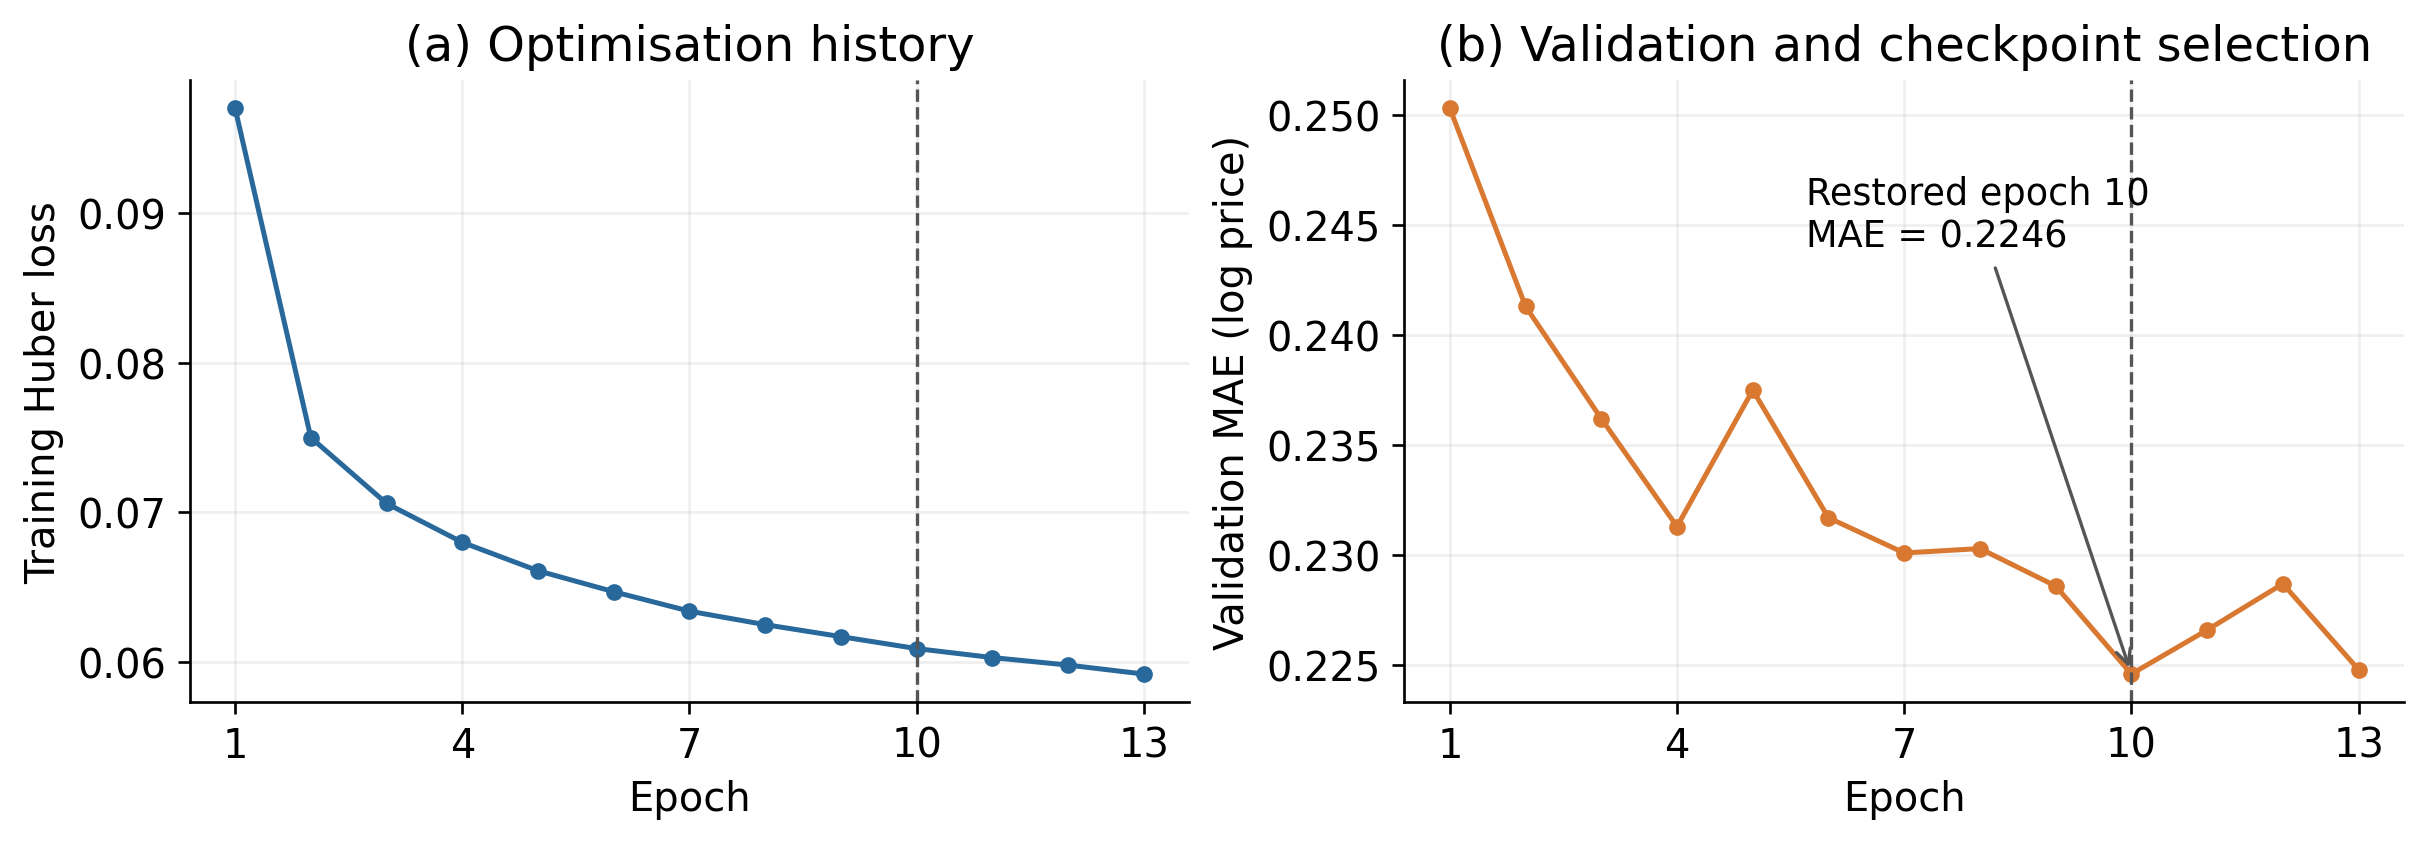
\includegraphics[width=0.92\textwidth]{figures/dl_mlp_training.png}
\caption[MLP training curves]{Tabular MLP training loss (Huber) and validation log-MAE over epochs. The dashed line marks the restored checkpoint at epoch 10.}
\label{fig:dl-mlp-training}
\end{figure}

\subsubsection{Value of Unstructured Listing Text}

Unstructured listing text provides substantial predictive information beyond structured attributes:
\begin{itemize}
  \item \textbf{Sparse representation (TF-IDF):} Horizontally concatenating TF-IDF unigrams~\cite{salton1988term} with structured features in Ridge regression reduces MAE by 13.9\% (from 5.730 to 4.935 billion VND) and raises $R^2$ from 0.551 to 0.632.
  \item \textbf{Stacked text prediction:} Feeding out-of-fold text-derived predictions into LightGBM~\cite{wolpert1992stacked} lowers MAE from 4.464 to 4.223 billion VND (a 5.4\% reduction), yielding the best single model in the study ($R^2=0.764$).
  \item \textbf{Pretrained language model (BamiBERT):} Fine-tuning BamiBERT~\cite{devlin2019bert} on raw titles and descriptions alone achieves an MAE of 4.355 billion VND and $R^2=0.763$. Operating entirely without structured tabular inputs, it surpasses all purely structured tabular models. This demonstrates that seller descriptions implicitly capture core property dimensions, location specifics, and amenity details.
\end{itemize}

\subsubsection{Model Ensembling and Blending}

Combining predictions through non-negative least squares on the validation set yields the lowest overall prediction error. Blending purely structured models (LightGBM, XGBoost, CatBoost, and MLP) achieves an MAE of 4.241 billion VND. Incorporating TF-IDF predictions reduces this to 4.025 billion VND, while adding BamiBERT drives it down to 3.699 billion VND.

\begin{figure}[H]
\centering
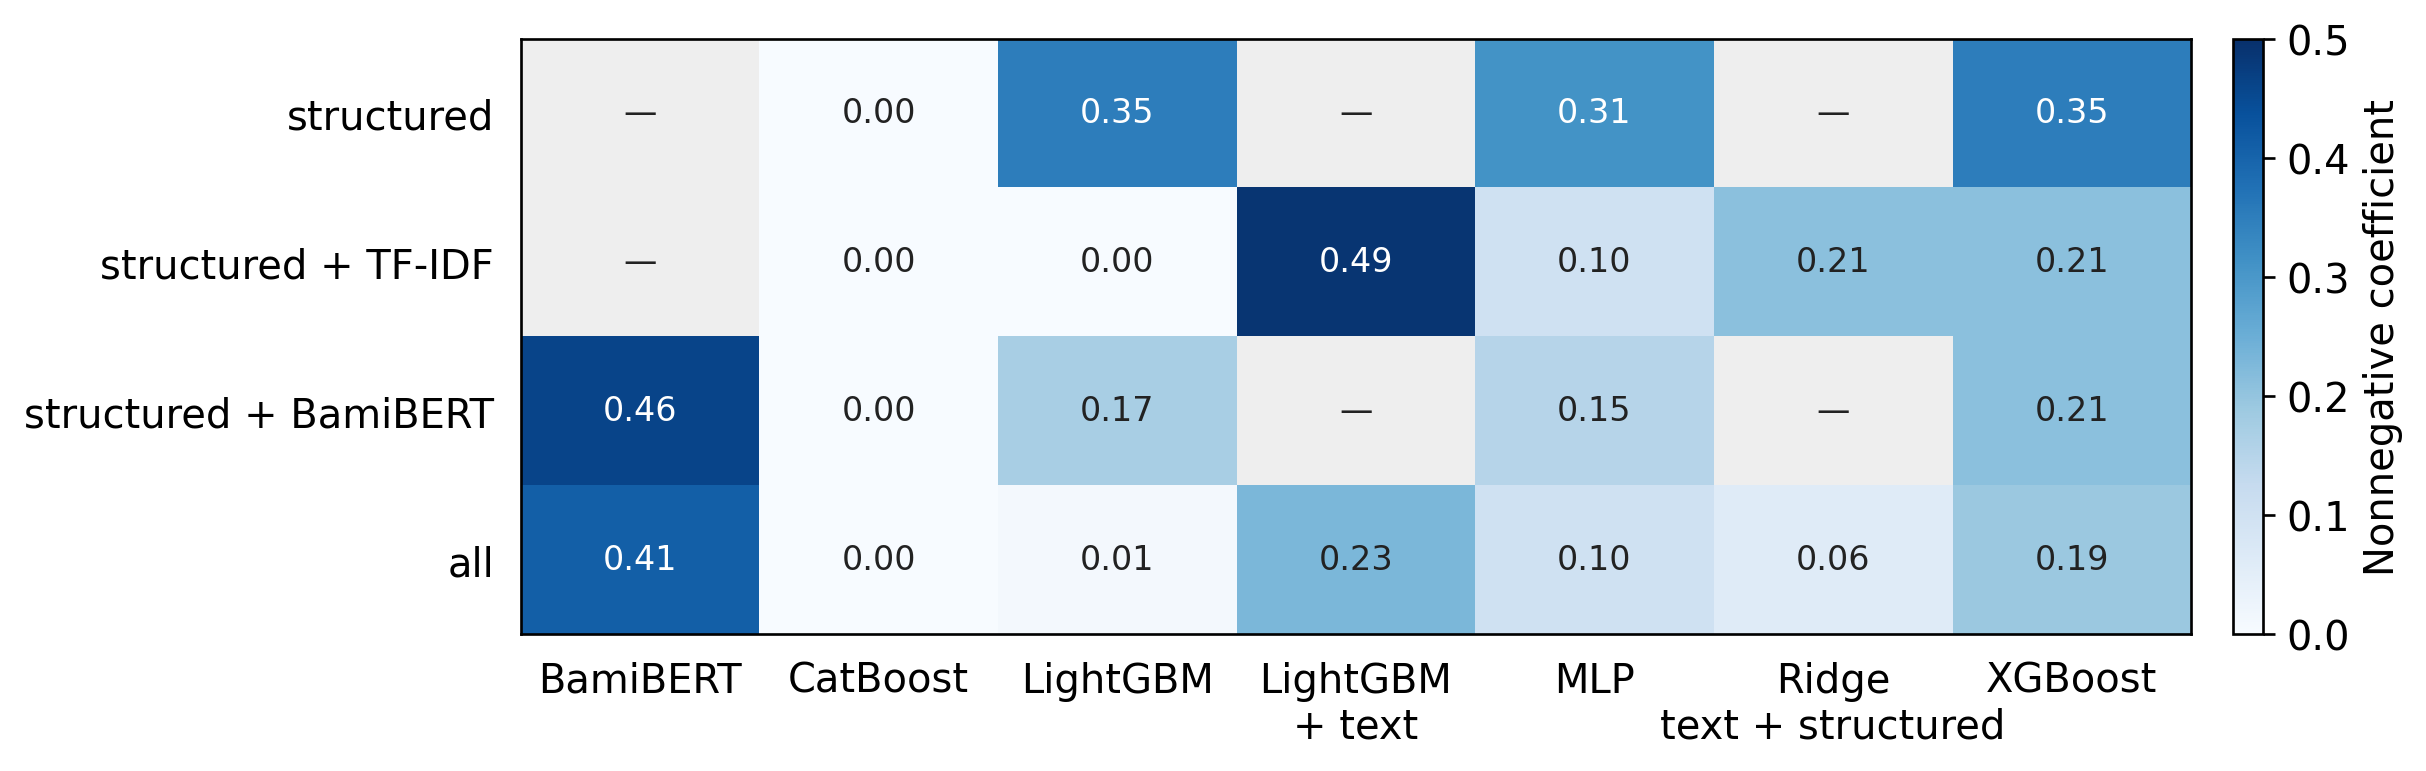
\includegraphics[width=0.92\textwidth]{figures/dl_ensemble_coefficients.png}
\caption[Validation-fitted blend weights]{Non-negative weights assigned to each base model across the four blending configurations (rounded to two decimals). Dashes denote excluded predictors.}
\label{fig:dl-blend-coefficients}
\end{figure}

Combining all seven models yields the optimal overall result: MAE 3.659 billion VND, RMSE 16.171 billion VND, $R^2=0.794$, and MAPE 21.70\%. This represents an 18.0\% error reduction relative to the structured LightGBM baseline. As shown in Figure~\ref{fig:dl-blend-coefficients}, the blend assigns dominant weights to BamiBERT (0.41), text-enhanced LightGBM (0.23), and XGBoost (0.19). Models drawing on complementary information sources (text vs.\ tabular) contribute far more diversity to the ensemble than combining multiple tabular models of the same family.

\subsection{Limitations}
\label{subsec:evaluation-limitations}

\paragraph{Target and population coverage.}
The target variable is the advertised asking price rather than a verified transaction price. In addition, sale and rental listings coexist without explicit labels. Geographically, approximately 71\% of the analytical dataset is concentrated in Hồ Chí Minh City and Hà Nội, limiting empirical generalization to smaller provinces.

\paragraph{Evaluation protocol.}
All findings are based on a single chronological train/validation/test partition. While this mimics forward-looking deployment, evaluating across multiple rolling temporal windows and constructing bootstrap confidence intervals would be required to establish statistical significance for small performance margins.

\paragraph{Text filtering.}
Although explicit monetary phrases were systematically removed from titles and descriptions, informal phrasing, abbreviations, or misspelled price mentions may remain in free text. Because BamiBERT retains numeric tokens, minor residual price leakage cannot be fully ruled out.

\endgroup
